\chapter{Concepts and Methods}
\label{chap:concepts_and_methods}
\section{Data Generation}
In order to build a model which is able to predict the behavior of parameterized algorithms, representative training data is necessary. As in many other ML applications, this data does not exist initially which is called the cold start problem \cite{Woltmann2021}. Solving this problem requires an adequate data generator producing representative integer values which then have to be labeled with the behavior of each considered algorithm i.e the compression rate and the compression runtime. Since all lightweight integer compression algorithms need integer sequences as input data, it is necessary to derive a representation of them. A common approach is the usage of \emph{bit width histograms} (bwhist) \cite{Damme2020, Woltmann2021}. In an integer sequence, every value has a different bitwidth maximum depending on the size of the value. A bwhist of a sequence consists of \emph{b} buckets where \emph{b} is equal to the amount of bits that are used to represent the integer values of the sequence. Every bucket contains the percentual share of a specific bit width of all sequence elements.

Woltmann et. al \cite{Woltmann2021} presented multiple ways to generate representative bwhists. They showed in their evaluation that the La-Ola generator performed reasonably well even though it is the most simple strategy. The generator starts with the bwhist having a full first bucket while all other buckets are empty. 
During each iteration step a fixed percentage (percentage shift) that has been determined previously is transferred to the next bucket. The process continues until the last bucket is filled completely. The amount of bwhists being generated is determined by the amount of buckets and the percentage shift according to equation \ref{eq:amount-of-bwhist-equation} where \emph{b} is the amount of buckets, \emph{s} the percentage shift, and \emph{n} the amount of bwhists:\\
\begin{equation} \label{eq:amount-of-bwhist-equation}
    n = \floor*{\frac{1}{s}} \cdot (b-1) + 1 
\end{equation}
\begin{figure}[h]
    \centering
    \begin{subfigure}{.5\textwidth}
      \centering
      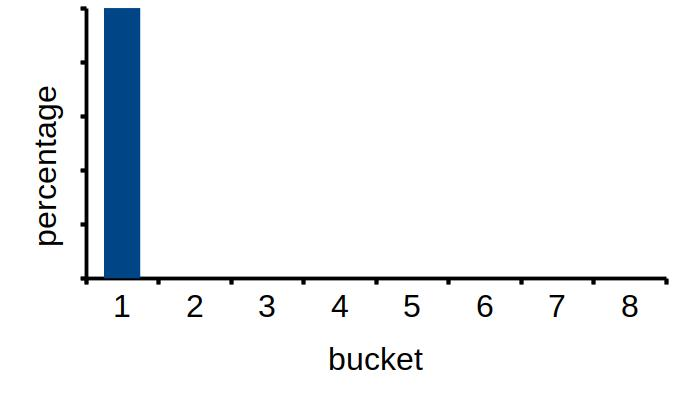
\includegraphics[scale = 0.4]{laola-1}
      \caption{bwhist 1}
    \end{subfigure}%
    \begin{subfigure}{.5\textwidth}
      \centering
      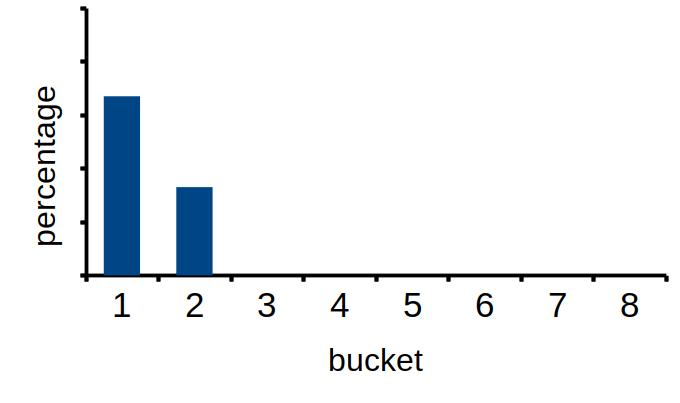
\includegraphics[scale = 0.4]{laola-2}
      \caption{bwhist 2}
    \end{subfigure}%
    \\
    \begin{subfigure}{.5\textwidth}
      \centering
      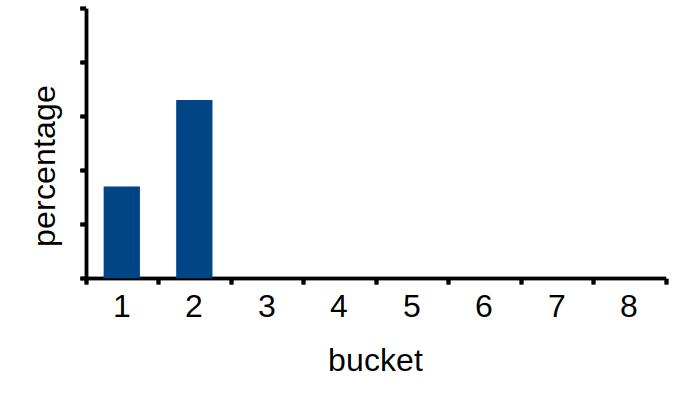
\includegraphics[scale = 0.4]{laola-3}
      \caption{bwhist 3}
    \end{subfigure}%
    \begin{subfigure}{.5\textwidth}
      \centering
      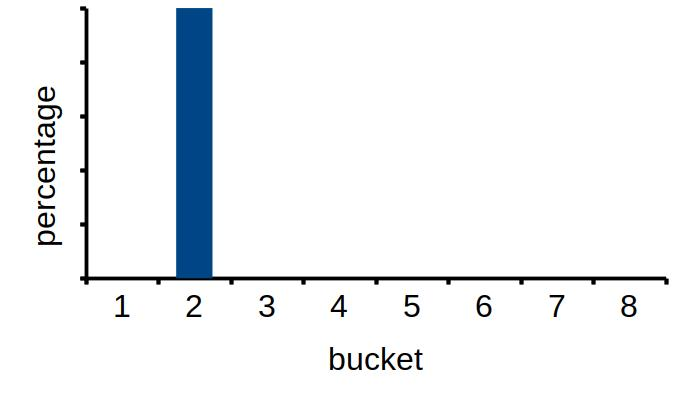
\includegraphics[scale = 0.4]{laola-4}
      \caption{bwhist 4}
    \end{subfigure}%
    \caption{La-Ola generation example for a 8-bit integer sequence and a percentage shift of 0,33.}
    \label{fig:laola-example}
\end{figure}

Figure \ref{fig:laola-example} shows the first four bwhists being generated for sequences of 8-bit integers with a percentage shift of 0,33. This La-Ola configuration would generate 22 bwhists. Due to the good ratio between simplicity and performance, we use the La-Ola approach for our data generation as well. After the bwhist generation, an integer sequence of arbitrary size can be derived.

In order to label the generated data, the implementation of the COLLATE-Metamodel \cite{Hildebrandt2017} was used as it supports multiple algorithms as well as different parameterizations. The current version of it includes \emph{StaticBP} and \emph{DynamicBP}. Therefore, only those two algorithms are considered, but the selection strategy for parameterizations can be extended for additional algorithms easily.\\
The framework supports the input format, the output format, the maximum bitwidth, and whether the sequence is sorted or not as parameters. As all of them except the output format are data-dependent, not every possible combination of parameters is valid. Therefore, only valid combinations are added to the source data before they are getting labeled.

\section{Feature Engineering}
Regarding ML, the process of feature engineering is considered as an important, but also most labor-consuming one \cite{Bengio2013}, as the quality of the model highly depends on the feature vectors it was trained with \cite{Heaton2016}.\\
After the generation of the bwhists and the integer sequences they are representing, it is necessary to derive features the ML model can be trained with. They can be divided in three classes. The first class contains features, that can be directly derived from the bwhist and have also been used for the selection strategy of Woltmann et. al \cite{Woltmann2021}. The second class contains features that have to be derived from the generated integer sequence. Class three is formed by features representing algorithm parameters.

\textbf{Class 1:}
\begin{itemize}[topsep=0pt]
    \itemsep0pt
    \item minBucket: The lowest bucket of the bwhist that contains a percentage higher than 0.
    \item maxBucket: The highest bucket of the bwhist that contains a percentage higher than 0.
    \item minPercentage: The lowest percentage of the bwhist a bucket contains. 
    \item maxPercentage: The highest percentage of the bwhist a bucket contains.
    \item averageBitwidth: The average bitwidth of the bwhist.
\end{itemize}
The average bitwidth is the weighted sum of the bitwidths the buckets are representing and its percentage.

\textbf{Class 2:}
\begin{itemize}[topsep=0pt]
    \itemsep0pt
    \item mean: The mean value of the integer sequence.
    \item stdev: The standard deviation of the integer sequence.
    \item skew: The skew of the integer sequence.
    \item kurtosis: The kurtosis of the integer sequence.
    \item isSorted: A boolean value indicating if the sequence is sorted or not.
\end{itemize}
The feature isSorted can be assigned to the following class as well, as it is also part of the algorithm parameterization.

\textbf{Class 3:}
\begin{itemize}[topsep=0pt]
    \itemsep0pt
    \item maxBitwidth: The maximum bitwidth of the integer sequence.
    \item inputFormat: The input format of every value in the integer sequence.
    \item outputFormat: The output format of every value in the integer sequence.
\end{itemize}
All classes combined lead to 13 features representing an integer sequence and algorithm parameterizations.

The COLLATE-Metamodel of Hildebrandt et. al \cite{Hildebrandt2017} supports on the one hand the measurement of the compression runtime which is the sum of the times for compression and decompression, and the compression rate on the other hand. We used both of them as target values by training one model for the compression rate and one for the compression runtime in order to compare them.

\section{Hyperparameter Tuning}
After the data generation and feature engineering process, it is necessary to train the model and tune the hyperparameters. Like Woltmann et. al \cite{Woltmann2021} we decided to use GB regression to build our ML model. In comparison to Neural Networks, the training phase of a GB model is less time-consuming. This is an important aspect for our use case as we need a ML model for every combination of algorithm and target value. Due to the consideration of the algorithms \emph{StaticBP} and \emph{DynamicBP} as well as the target values compression runtime and compression rate, four models have to be trained. Additionally, GB regression has certain hyper parameters. The number of weak learners i.e decision trees and the maximum depth per decision tree are the parameters mainly influencing the model's quality \cite{Woltmann2021}. Regarding the number of decision trees, we considered the search space \(T = [10,100] \cup{[200]}\) with a step size of 10 for the first interval. For the maximum depth per tree, the search space \(D = [3,12]\) was used.

Based on both sets, the size of the whole two-dimensional search space \emph{s} is the product of the cardinalities of \emph{T} and \emph{D} as shown in equation \ref{eq:size-of-search-space}.
\begin{equation} \label{eq:size-of-search-space}
    s = |T| \cdot |D| = 110 
\end{equation}
In order to compare the quality of the trained models, we decided to use the SMAPE metric which is the Symmetric Mean Absolute Percentage Error between a set \emph{P} of predicted values and a set \emph{A} of actual values. It is defined as follows:
\begin{equation} \label{eq:smape}
    SMAPE(A,P) = \frac{200\%}{n} \sum_{i = 1}^{n} \frac{|P_{i} - A_{i}|}{|A_{i}| + |P_{i}|}
\end{equation}
\begin{figure}[h]
    \centering
    \begin{subfigure}{.5\textwidth}
      \centering
      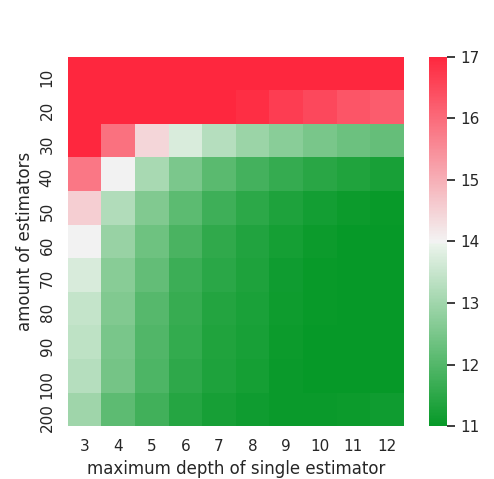
\includegraphics[scale=0.5]{ht_heatmap_dynamic_duration}
      \caption{\emph{DynBP}}
    \end{subfigure}%
    \begin{subfigure}{.5\textwidth}
      \centering
      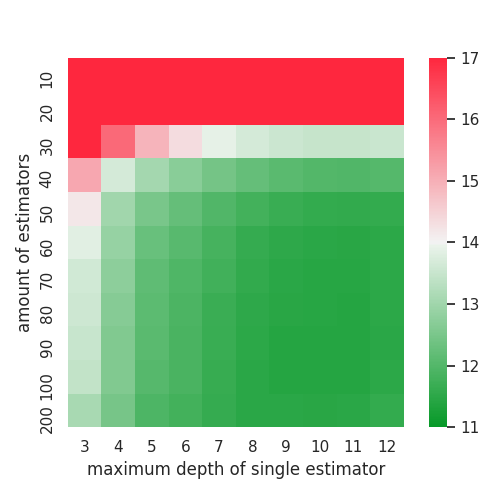
\includegraphics[scale=0.5]{ht_heatmap_static_duration}
      \caption{\emph{StatBP}}
    \end{subfigure}%
    \caption{Hyperparameter tuning results (SMAPE in \%, compression runtime as target value).}
    \label{fig:hyperparameter-heatmap-duration}
\end{figure}
\begin{figure}[h]
    \centering
    \begin{subfigure}{.5\textwidth}
      \centering
      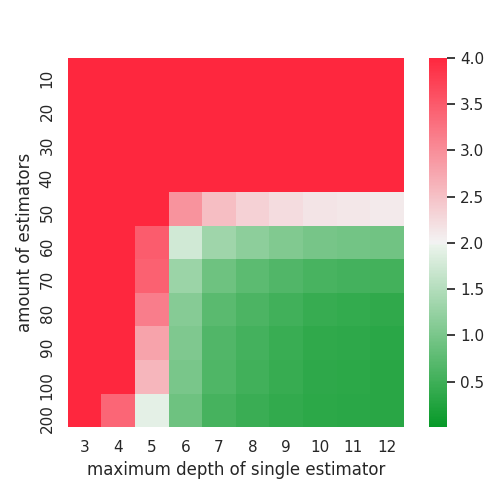
\includegraphics[scale=0.5]{ht_heatmap_dynamic_rate}
      \caption{\emph{DynBP}}
    \end{subfigure}%
    \begin{subfigure}{.5\textwidth}
      \centering
      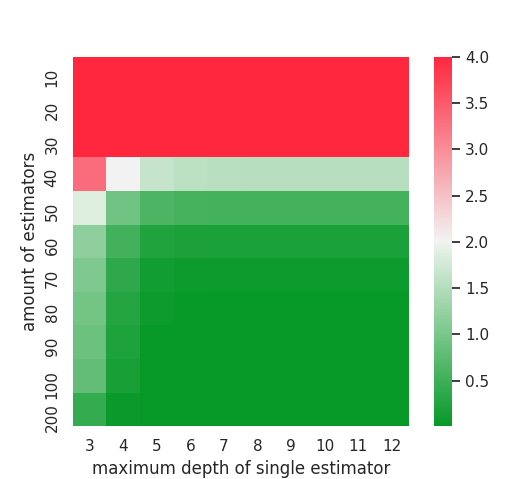
\includegraphics[scale=0.5]{ht_heatmap_static_rate}
      \caption{\emph{StatBP}}
    \end{subfigure}%
    \caption{Hyperparameter tuning results (SMAPE in \%, compression rate as target value.)}
    \label{fig:hyperparameter-heatmap-compression-rate}
\end{figure}

The hyperparameter tuning process has shown that for \emph{DynamicBP}, 80 estimators and a maximum depth per tree of 10 for both, the compression rate and the compression runtime lead to reasonably good SMAPE values while not overfitting the model.
For \emph{StaticBP},  80 estimators and a maximum depth per tree of 9 for the compression runtime and 80 estimators and a maximum depth of 6 for the compression rate lead to the best results.

\section{Conclusion}
Based on the presented methods of data generation, feature engineering, and hyperparameter tuning, a set of ML models can be trained with representative data which is the core element of the \emph{Learned Selection Strategy For Lightweight Integer Compression Algorithm Parameterizations}. Having a sequence of integers, the bwhist of it can directly be derived. Given this representation, it is possible to predict the best-fitting algorithm and its parameters by passing every possible input combination to each algorithm model and selecting the one with the best compression runtime or compression rate. 

As all of the concepts are general abstractions, a specific implementation is necessary for data generation, data labeling and model training on the one hand, as well as validation and forward passing on the other hand.  
